\documentclass[Main]{subfiles}
\begin{document}

\chapter{Geodesic Fields}
	%mettere nell'intro una breve introduzione al problema geodetico nell'approccio standard della geometria riemmaniana
	In the context of differential geometry, \emph{geodesic curves} are a generalization of \emph{straight lines}  in the sense of self-parallel curves.
	%Definizione di geodetica su varietà con connessione
	Considering a differential manifold $M$ endowed with an affine connection $\nabla$ we define:
	\begin{definition}[Geodesic]
		A curve \danger\footnote{Devo dire smooth o piecewise? }
		$\gamma:[a,b]\rightarrow M$ such that:
		\begin{equation}
			\nabla_{\dot{\gamma}}\dot{\gamma} =0
		\end{equation}
		where $\dot{\gamma}^\mu \coloneqq \frac{d \gamma^\mu}{d t}$ is the tangent vector to the curve.
	\end{definition}
	\begin{notationfix}
		In local chart the previous equation assume the popular expression:
		\begin{equation}\label{GeodesicEquation}
			\ddot{\gamma}^i + \Gamma^i_{\, j k} \dot{\gamma}^j \dot{\gamma}^k = 0
		\end{equation}
		Where $ \Gamma^i_{\, j k}$ is the coordinate representation of the Christoffel symbols of the connection.
	\end{notationfix}
	%Definizione metrica di geodetica su varietà riemmaniana( con connessione di levi civita)
	\vspace{4mm}
	
	In presence of a pseudo-Riemannian metric is possible to present the geodesic in a metric sense i.e. as the curve  which extremizes the \emph{Energy Functional}\footnote{Remember that for arc-length parametrized curves the Energy functional coincide with the length functional.\cite[Lemma $1.4.2$ ]{Jost2005}}:
	\begin{definition}[Energy functional]
  	\begin{equation}\label{EnergyFunctional}
 		E(\gamma) \coloneqq \int_a^b \left\Vert \frac{d \gamma}{dt} (t)\right\Vert^2 dt
 	\end{equation}
\end{definition} 	
	Considering only the proper variation (that keep the end-point fixed), the extremum condition corresponds to equation \ref{GeodesicEquation} where $\nabla$ is the unique Levi-Civita connection (torsion-free and metric-compatible).
	%Problema di Jacobi, deviazione geodetica e legame alla curvatura
	\vspace{4mm}
	
	In general relativity the problem of the geodesic equation linearization, named \emph{Jacobi equations} takes a central role. \footnote{Usually in this context takes the name of \emph{Geodesic deviation} problem\cite[pag. 46]{Wald1984}.}
	
\begin{Warning}
	(nel file di ripasso di geometria riemmaniana ho scritto gran parte delle definizione conviene vedere cosa mi serve effettivamente...
	Di certo mi avvalgo della seguente  equazione
\end{Warning}
	
	\begin{notationfix}
		In local charts the Jacobi fields along the geodesic $\gamma$ solve a linear O.D.E.:
		\begin{equation}\label{JacobiEquationComponents}
			\big( X''\big)^\mu + R^\mu_{i \alpha \j} T^i X^\alpha T^j =0
		\end{equation}
		where:
		\begin{itemize}
			\item $\big(X'\big)^\mu \coloneqq \big( \nabla_{\dot{\gamma}(t)} X\big)^\mu$ is the covariant derivative along the curve $\gamma$.
			\item $T \equiv \dot{\gamma}(t)$ stands for the tangent vector to the curve $\gamma$.
		\end{itemize}
	
	\end{notationfix}
	
	
	
	
	The rest of this chapter will be dedicated to presenting the physical approach to the Geodesic.


\section{Geodesic Problem as a Mechanical Systems}\label{GeodesicMechanics}
	% Da quanto detto in introduzione ha un odore molto forte il legame  dell'equazione geodetica con l'equazione del moto di un punto su una varietà e dell' funzionale lunghezza come versione con il prinicpio di minima azione
	The basic idea is very simple, portray the geodesic curve as the natural motion of a free particle constrained on the Pseudo-Riemannian manifold $Q$.
	
	\begin{Warning}
	obvious enough this problem can be seen as a generalization of the calculation of the motions of free falling parcticles
	In terms of general relativity this problem can be instantly recognized as the derivation of the free-falling particles motion.
	
	However, there is no lack of alternative viewpoints .
	The framework of the classical Geometric Mechanics teach us to picture the "static" configurations of a constrained, complex, classical system as a point on the \emph{Configuration space} manifold. According to that, the geodesic motion can be seen as a realization of a particular dynamics on each mechanical system endowed with a pseudo-Riemannian configuration space\footnote{Such systems can be depicted as "geodesic" even in presence of a position-dependant potential.\cite[Cap 3.7]{Abraham1978}}.
	\end{Warning}


	% Q è la varietà riemmanian in esame, eccc. vedi pag 223  e successive del fomm (direi di dare per assodato tutto il contesto di meccanica geometrica che mi sono studiato nei primi mesi della tesi ma credo non sia il caso di mettere per esteso qui, al massimo solo linkarlo

	\begin{theorem}[Geodesic Motion]
		The geodesics on the Pseudo-Riemmanian manifold $(Q,g)$ are the natural motions of the ordinary Lagrangian system $(Q, L)$ where:
		\begin{equation}
			L(V_q) \coloneqq \frac{1}{2} g_q(V,V)
		\end{equation}
	\end{theorem}	
	\begin{proof}
		 The Euler-Lagrange equation of $L$ coincides with the geodesic equation \ref{GeodesicEquation}.
		 \danger.. è sul quaderno non so se metterla
	\end{proof}

	\begin{observation}
		The geodesic system is not simply Lagrangian but also Hamiltonian.
		This property follows from the hyperregularity\cite{Abraham1978} of $L$.
		
		\begin{Warning}
		Anyway we will neglect this fact inasmuch in what follows only the Lagrangian character assumes a role.
		\end{Warning}
	\end{observation}


	%Qualsiasi sistema di mqo come il precedente può essere visto come un sistema campo.
	As shown in chapter 2, every system with discrete degrees of freedom can be seen as the trivial field system.
	From that follows the alternative characterization of geodesic as a lagrangian field:
	\begin{corollary}[Geodesic field]
		The geodesics on the Pseudo-Riemmanian manifold $(Q,g)$ can be seen as the \emph{Dynamical Configurations} of the lagrangian field system $(E,\Lagrangian)$ where:
		\begin{itemize}
			\item $E=(Q\times\Real, \pi, \Real)$ trivial smooth bundle on the real line.
			\item $\Lagrangian[\gamma] = \frac{1}{2} g(\dot{\gamma},\dot{\gamma})(t) dt$
		\end{itemize}
	\end{corollary}
	\begin{proof}
		Is simple application of the correspondence seen in chapter \ref{MechanicsAsAField}.
	\end{proof}
	
	From this perspective is clear that the Energy Functional can be seen as the action in the geodesic field dynamics and equation \ref{GeodesicEquation} is nothing more than the motion equation according to the \emph{least action principle}.

		\begin{figure}[h!]
				  \centering
   	%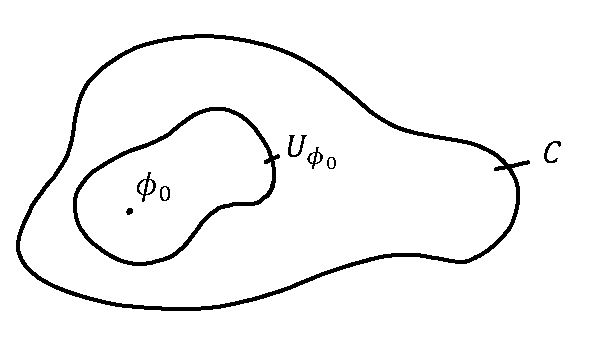
\includegraphics[width=0.5\textwidth]{Pictures/Linearization} 
   	  \caption{Impressionistic view of the geometric mechanics structure.}
		\end{figure}		


\section{Peierls Bracket of the Geodesic field}
	The local coordinate expression of the lagrangian density of the geodesic field results:
	\begin{equation}
		\Lagrangian\big(t,\gamma^i(t), \dot{\gamma}^i(t) \big)\coloneqq \frac{1}{2}g_{\mu,\nu}\big(\gamma^i(t))\dot{\gamma}^\mu \dot{\gamma}^\nu
	\end{equation}		
	this is highly non-linear. Explicitly is quadratic in the velocity components $\dot{\gamma}^i$ and implicitly, through $g_{\mu\nu}(\gamma^i(t))$, is non-polynomial in coordinate $\gamma^i$.
	
	As show in section \ref{•}, for this type of systems, the calculation of Peierls bracket can be realized only locally around a predetermined solution.
	Let's repeat the Peierls' procedure for the system under investigation.
	
	\begin{Warning}
	Introduzione da rividere, dimostro che l'operatore linearizzato senza termine inomogeneo corrisponde all'equazione di Jacobi vera e propria mentre con termine inomogeneo dato dalle E-P del disturbo da l'equazione che definisce la perturbazione ritardata e anticipata.
	\end{Warning}

	As a consequence of our introduction on the geodesic as a field, we can state the unperturbed dynamic as a L.P.D.O :
		\begin{equation}
			Q_\Lagrangian \big(q^\mu 	\big)= \biggr[\ddot{q}^\mu + \Gamma^\mu_{\, i j}\dot{q}^i \dot{q}^j	\biggr]
		\end{equation}
	where $\dot{q}^\mu = \frac{d}{dt}q^\mu(t)=\dot{q}^i\partial_i q^\mu$.
	
	A linear variation of $q_0^\mu +\epsilon \eta^\mu$ constructed from the coordinate representation $q_0^\mu$ of the geodesic $\gamma_0 \in \Sol$, solves the original motion equations when
	\begin{equation}\label{GeodesicJacobation1}
		Q_\Lagrangian \big( q_0^\mu +\epsilon \eta^\mu \big) = \frac{d^2}{dt^2}\biggr( q_0^\mu +\epsilon \eta^\mu \biggr) +
		\biggr[ \Gamma^\mu_{\, i j}\big( \vec{q_0} + \epsilon \vec{\eta}\big) \biggr]\biggr(\dot{q_0}^i +\epsilon \dot{\eta}^i \biggr)\biggr(\dot{q_0}^j +\epsilon \dot{\eta}^j \biggr) = 0 \mbeq o(\epsilon)
	\end{equation}
	If we consider only the first order in the parameter $\epsilon$ we can expand the expression of the Christoffel symbols:
	\begin{displaymath}
		\biggr[ \Gamma^\mu_{\, i j}\big( \vec{q_0} + \epsilon \vec{\eta}\big) \biggr] =
		\biggr[ \Gamma^\mu_{\, i j}( \vec{q_0}) + \epsilon \eta^\alpha\big( \partial_\alpha  \Gamma^\mu_{\, i j} \big)\biggr\vert_{\vec{q_0}} + o(\epsilon) \biggr]
	\end{displaymath}	 
	
	Collecting all the terms in equation \ref{GeodesicJacobation1} up the first order in $\epsilon$ follows a condition on the perturbation:
	\begin{displaymath}
	0 = \ddot{\eta}^\mu + \eta^\alpha\big( \partial_\alpha  \Gamma^\mu_{\, i j} \big)\biggr\vert_{\vec{q_0}} \dot{q_0}^i \dot{q_0}^j  +  \Gamma^\mu_{\, i j} \big(\dot{\eta}^i \dot{q_0}^j + \dot{q_0}^i \dot{\eta}^j \big)=
	=\biggr\{ g^\mu_{\,\alpha} \frac{d^2}{dt^2} +
	 \Gamma^\mu_{\, i \alpha}(\vec{q_0})\big[2 \dot{q_0}^i \frac{d}{dt} \big] + 
\big[ \partial_\alpha  \big] \biggr\} \eta^\alpha	 
	\end{displaymath}		
	
	
	\begin{Warning}
	Da dire: espressione in coordinate della lagrangiana, è altmente non lineare perchè implicitamente è $g_{\mu\nu}(\gamma^i(t))$ non polinomiale in $\gamma^i$ ed esplicitamente è quadratica, Mostrare esplicitamente che l'equazione di jacobi per il sistema è effittivamente l'equjazione di jacobi ( questo è triviale se vedi come definisce il campo di jacobi jurgen 
	\end{Warning}	


	
	

\subsection{Example: Geodesic field on FRW space-time.}
	% qui i conti li devo ancora fare, l'idea è che le metriche possono essere diagonalizzate risulta un sistema di equazioni del moto ode disaccoppiate di cui posso calcolare la funzione di green come indicato nelle dispense che trattano il calcolo di green per le ode.
	%se ho l'operatore di green posso calcolare in esplicito le peierls

\section{Algebraic quantization of the Geodesic Field}
	\begin{Warning}
	va ripetuto che la geodetica è non lineare quindi ciò che effettivamente si quantizza è jacobi lungo una prefissata geodetica. questo è un campo lineare.
	\end{Warning}
	
	\begin{Warning}
	INtro: paragrafo sul quaderno: "qual'è l'interesse che spinge a quantizzare questo sistema "Campo di Jacobi"?
	\end{Warning}

	\begin{Warning}
		Disclaimer: Non approfondisco più di tanto gli step di quantizzazione vera e propria. il ruolo di peierls è nel prequantistico, definisce il bracket che poi va implementato sull'algebra. Una volta decisa la parentesi la macchinetta procede in automatico.
	\end{Warning}

\subsection{Peierls Approach}
		\begin{Warning}
		Paragrafo sul Quaderno: ...
	\end{Warning}

\subsection{Inital data Approach}
	\begin{Warning}
		Ancora su fogli di Brutta!
	\end{Warning}

\section{Interpretations??????}
	\begin{Warning}
		Speriamo bene.. :S
	\end{Warning}

\end{document}
